\subsection{Method 1 : Perceptron}

The first model was a a simple perceptron with 2 inputs which were based on [insert reference to paper here]. The inputs chosen measured the semantic similarity and the word order information of the 2 sentences.

\subsubsection{Words Similarity}
A \textbf{path length} between 2 words is the number of synsets we visit from one word to another. For example, in the figure below, to get from boy to girl we have to visit boy - male - person - female - girl. Therefore, the path length of 'boy' and 'girl' is 4. 'Person' is called the subsumer of 'boy' and 'girl'. If there are more than 1 path, we will consider the shortest path and the corresponding subsumer is called the \textbf{lowest subsumer}.

\begin{center}
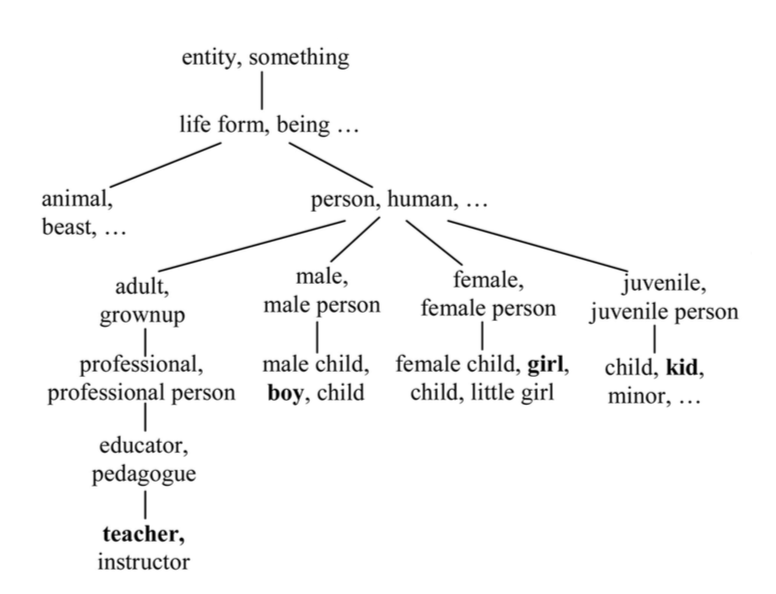
\includegraphics[scale=0.7]{Synset_tree}
\end{center}

Let $l$ denote the shortest path and $h$ denote the depth of the lowest subsumer. The similarity between 2 words $w_1$ and $w_2$ is therefore measured by 
\begin{equation*}
s(w_1, w_2) = f_1(l) f_2(h)
\end{equation*}
where $\alpha, \beta \in [0,1]$ and 
\begin{align*}
	f_1(l)		&= e^{-\alpha l} \\
	f_2(h)	&= \frac{e^{\beta h} - e^{-\beta h}}{e^{\beta h} + e^{-\beta h}} \\
\end{align*}

\subsubsection{Semantic Similarity}
Let $T_1$ and $T_2$ be the 2 sentences and T is a set of distinct words in T1 and T2. For each sentence, we will calculate the vector $s_k$ which the same length as T. For each word $w_i$ in T, we assign 1 to the corresponding element in $s_k$ if $w_i$ is in $T_k$ and $\mu_i$ otherwise. $\mu_i$ is the similarity score between $w_i$ and the most similar word in $T_k$ calculated based on the similarity score above. Once $s_1$ and $s_2$ are calculated, the overall semantic similarity score is calculated by 
\begin{equation*}
	S_s = \frac{s_1. s_2}{||s_1||.||s2||}
\end{equation*}

\subsubsection{Word Order}
Similar to the semantic similarity, we calculate the vectors $r_1$ and $r_2$ for each of the sentences. For each word $w_i$ in T, we set the $i^{th}$ element in $r_k$ to equal to the position of $w_i$ in $T_k$. If $w_i$ is not in $T_k$ then we find the most similar word in $T_k$ and assign the position of that word instead.

For both word order and semantic similarity measure, we define a threshold for the case where $w_i$ is not in $T_k$. If the similarity score between $w_i$ and the most similar word is less than the threshold, 0 will be assigned instead.

For the word order, the overall score is calculated by 
\begin{equation*}
	S_r = 1 - \frac{||r_1 - r_2||}{||r_1 + r_2||}
\end{equation*}